\chapter{Empirical Analysis}
\label{chap:empirical_analysis}

\subsection{Overview of the Dataset}
The dataset reveals a highly concentrated landscape of offshore activities. This concentration is particularly stark when examining the jurisdictions of incorporation, where a mere 15 countries account for approximately 98\% of all incorporated entities.

\subsubsection{Concentration of Relevant Elements}
Figure \ref{fig:preliminary_geography_overview} provides a visual overview of this geographical concentration.
\begin{figure}[htbp]
    \centering
    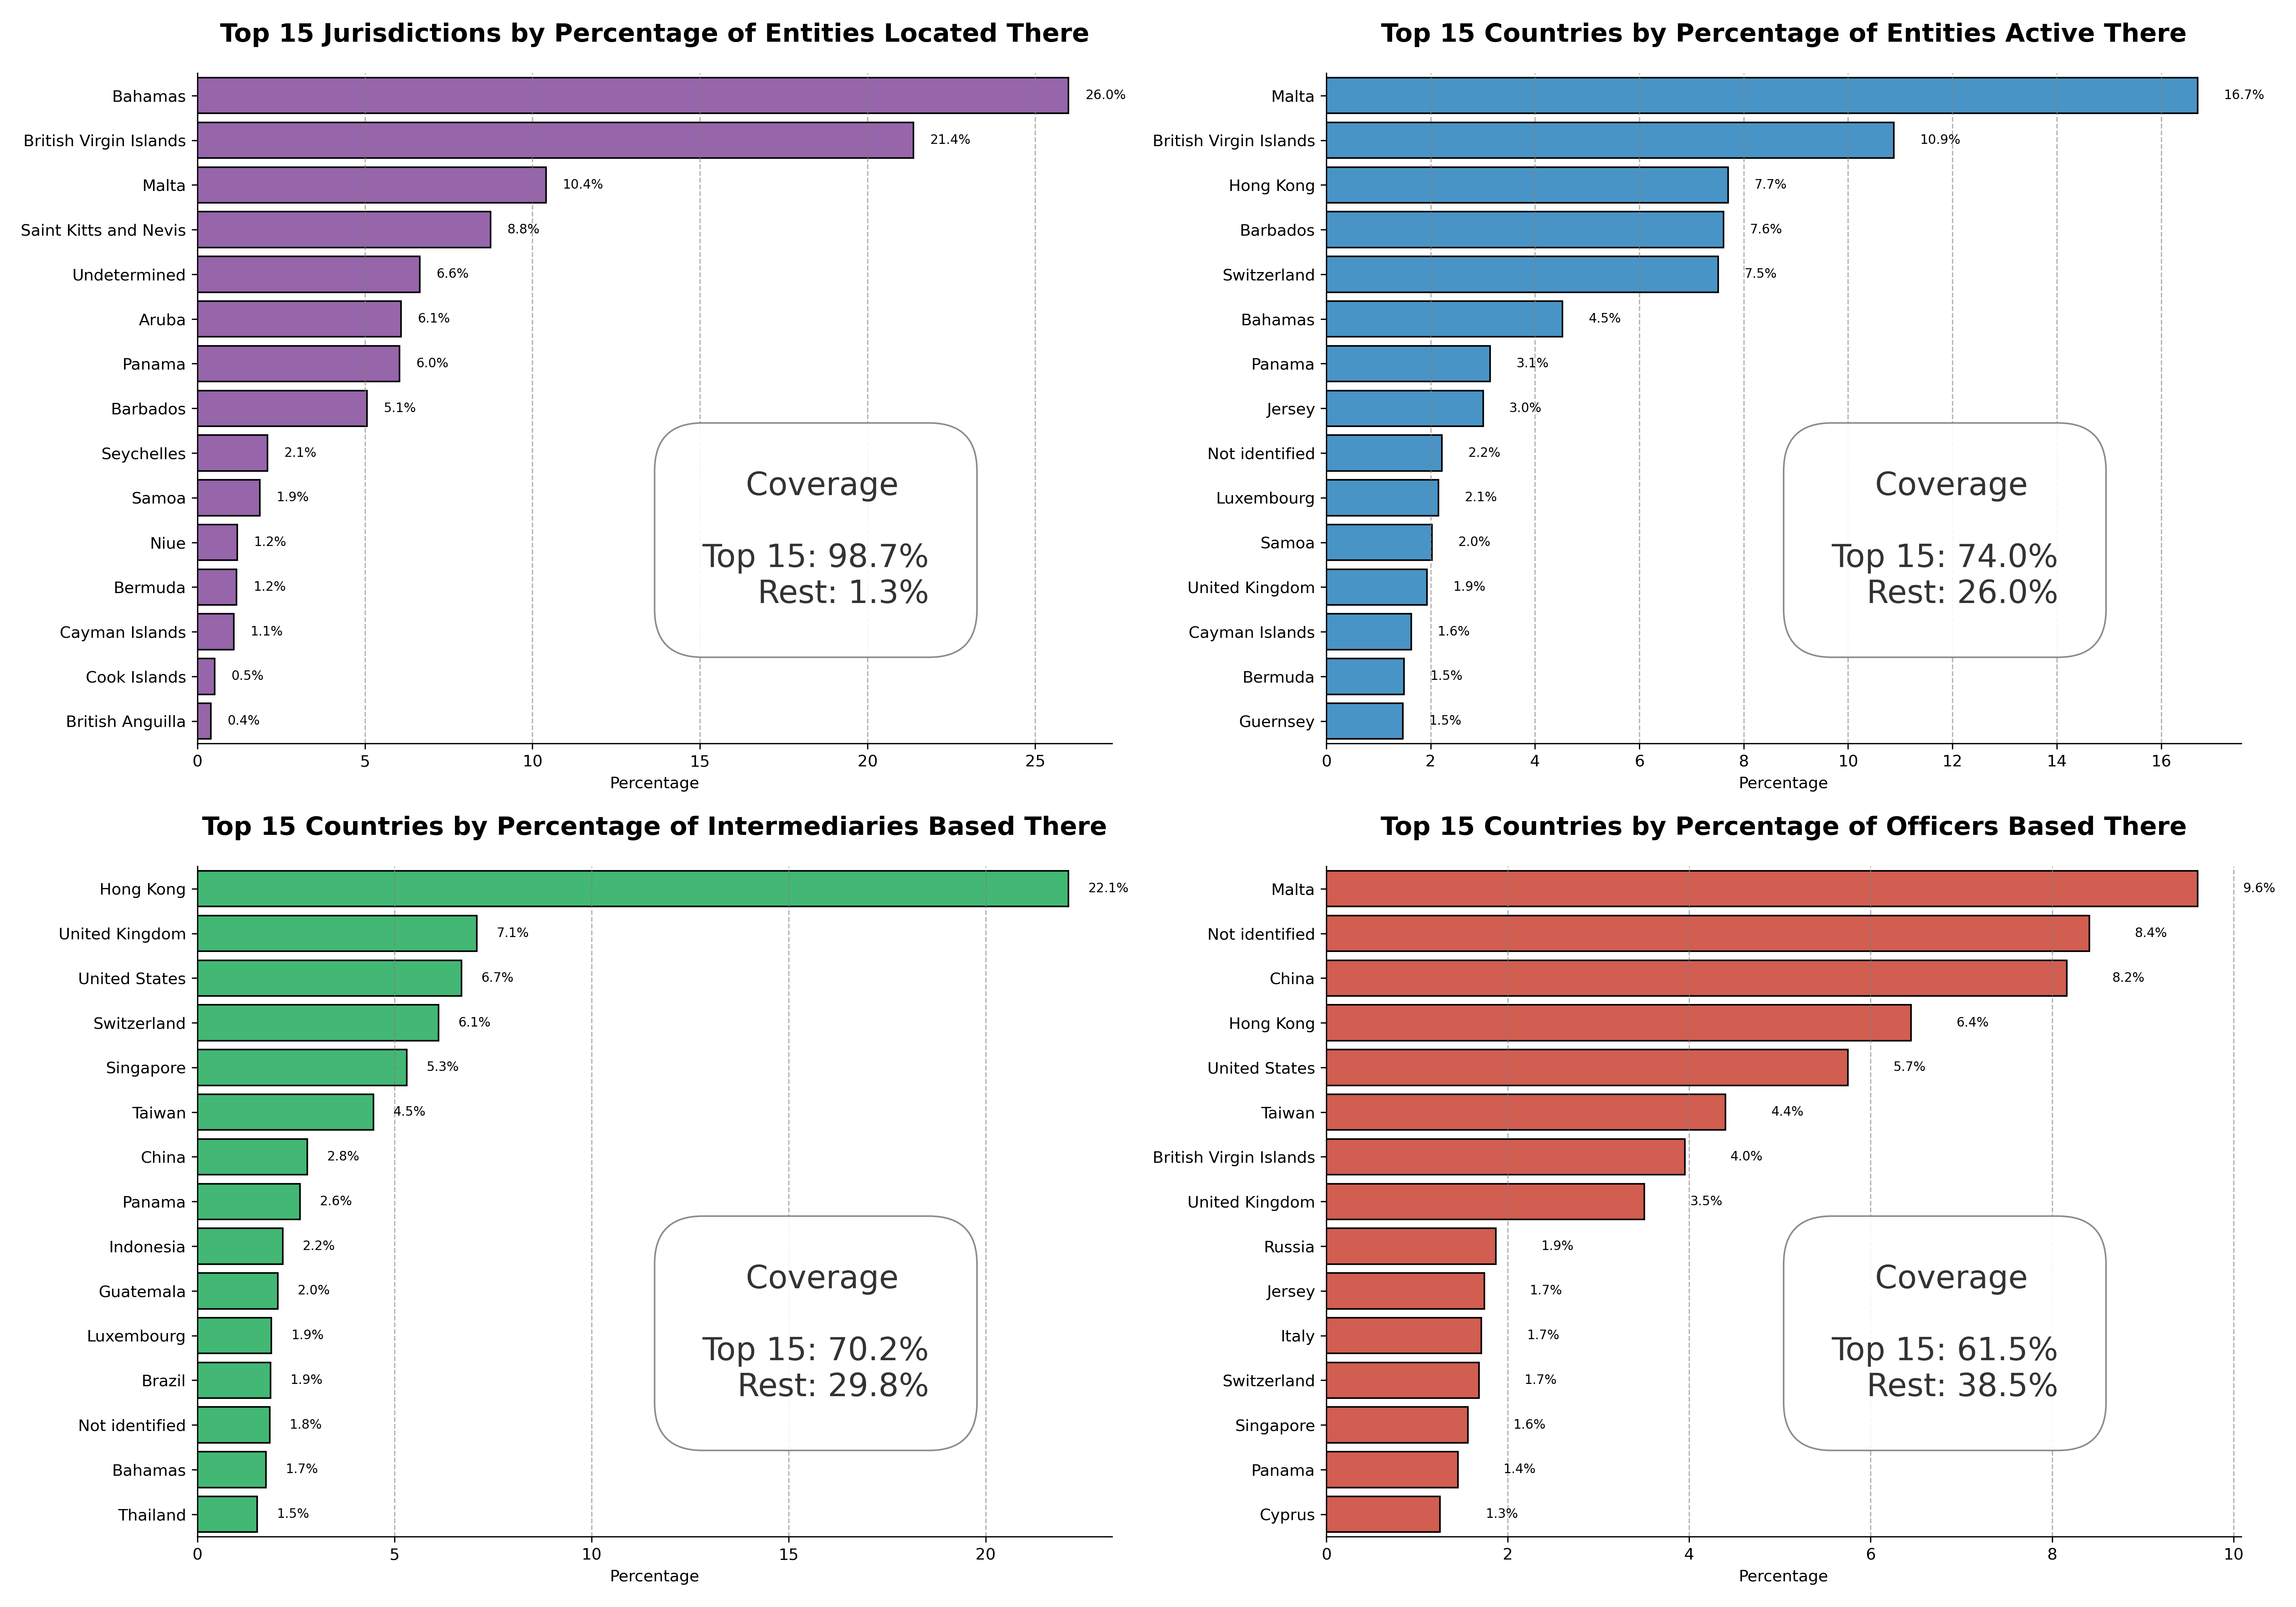
\includegraphics[width=0.8\textwidth]{Preliminary_Geography_Overview.png}
    \caption{Geographical Concentration of Entities and Intermediaries}
    \label{fig:preliminary_geography_overview}
\end{figure}

\subsubsection{Degree Distribution of Intermediaries}
A recurring theme within this analysis is the prevalence of power-law-like distributions. This is evident in the degree distribution of intermediaries (Figure \ref{fig:preliminary_powerlaw_fit}), which indicates that a small number of intermediaries are connected to a large number of entities, while most intermediaries have few connections. A formal comparison between a power-law and a log-normal distribution for the intermediary degree data yields a log-likelihood ratio $R = 57.0287$ with a $p$-value $< 0.0001$, suggesting a better fit for the power-law model or at least a heavy-tailed distribution. This characteristic underpins much of the thesis.

\begin{figure}[htbp]
    \centering
    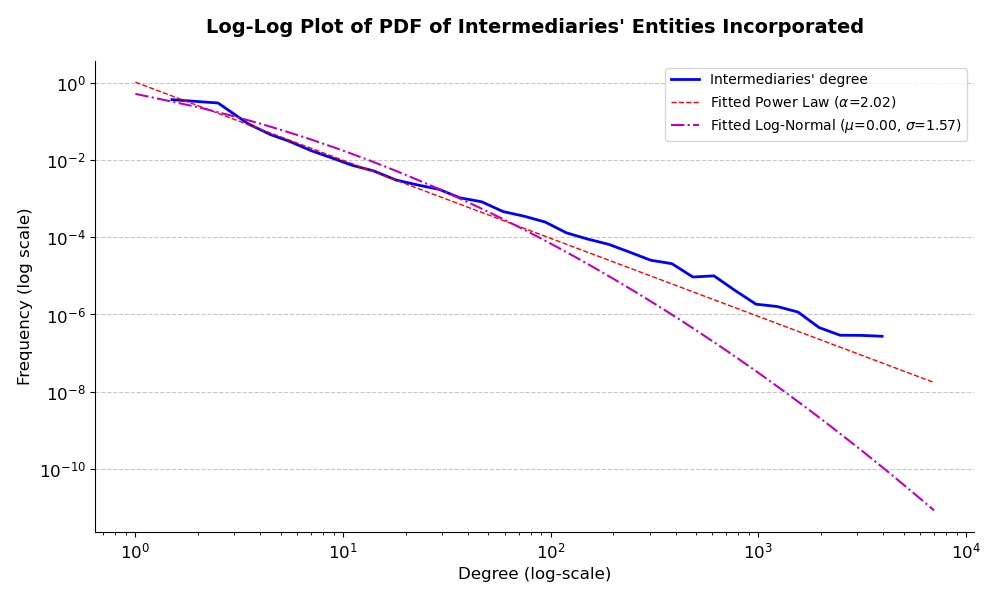
\includegraphics[width=0.8\textwidth]{Preliminary_Powerlaw_Fit.png}
    \caption{Degree Distribution of Intermediaries and Power-Law Fit}
    \label{fig:preliminary_powerlaw_fit}
\end{figure}

\subsection{Geographical Specialisation}
This section delves into the geographical patterns of intermediaries, examining their client locations and the jurisdictions they utilize for incorporation.

\subsubsection{Intermediary Specialisation at the Country Level}
When intermediaries are aggregated at the country level, distinct patterns emerge, as illustrated in Figures \ref{fig:geography_country_heatmaps_top5} through \ref{fig:geography_country_heatmaps_top11_15}. Intermediaries demonstrate a strong proclivity for serving clients from their own country. However, their choice of incorporation jurisdictions is more diverse. The entropy of jurisdictions used for incorporation by a country's intermediaries is significantly higher than the entropy of the countries where their clients' entities have their main activity (Figure \ref{fig:geography_country_level_entropy_distribution}). This suggests that while client bases are often geographically focused, the selection of incorporation jurisdictions is more globally dispersed, albeit concentrated within a relatively small number of preferred offshore jurisdictions.

A two-sample Kolmogorov-Smirnov test formally confirms that the distributions of client country entropy and incorporation jurisdiction entropy are significantly different.

\begin{figure}[htbp]
    \centering
    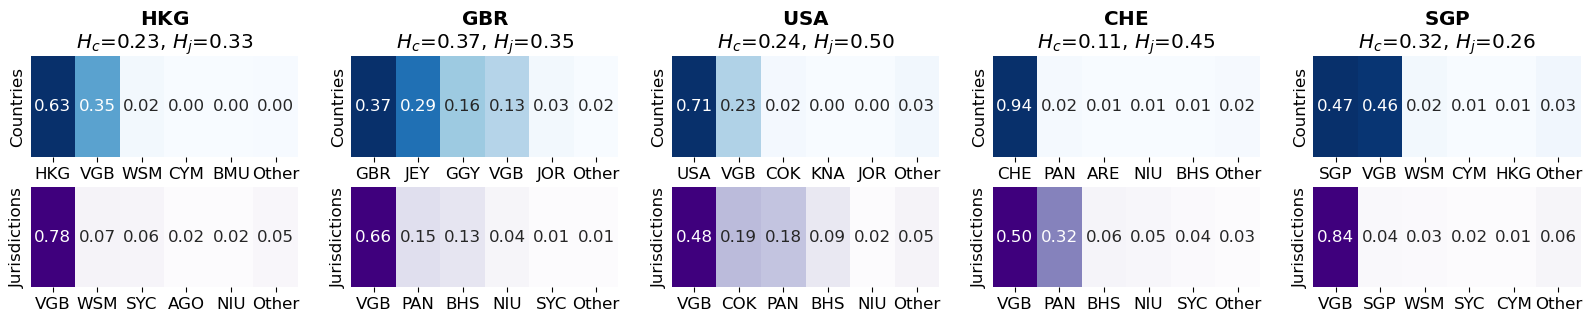
\includegraphics[width=0.8\textwidth]{Geography_Country_Heatmaps_Top5.png}
    \label{fig:geography_country_heatmaps_top5}
\end{figure}

\begin{figure}[htbp]
    \centering
    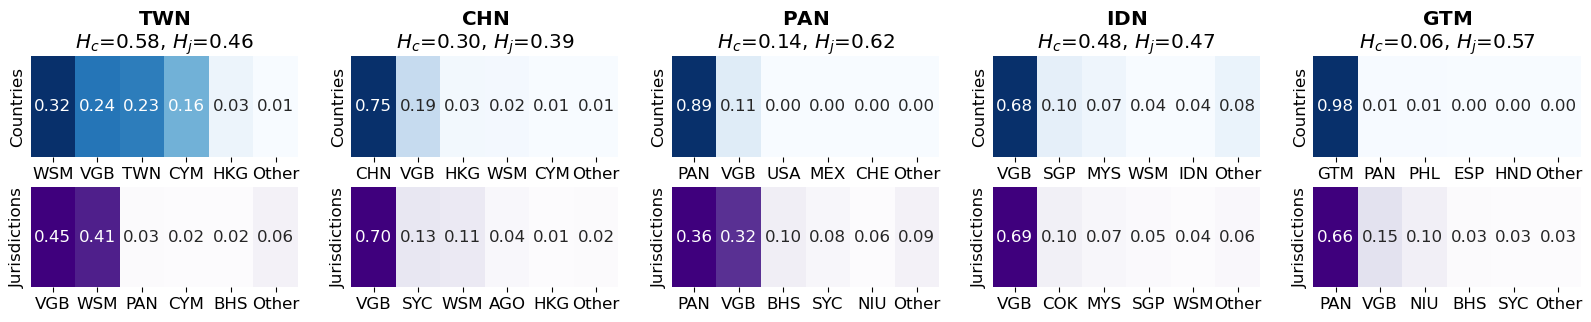
\includegraphics[width=0.8\textwidth]{Geography_Country_Heatmaps_Top6_10.png}
    \label{fig:geography_country_heatmaps_top6_10}
\end{figure}

\begin{figure}[htbp]
    \centering
    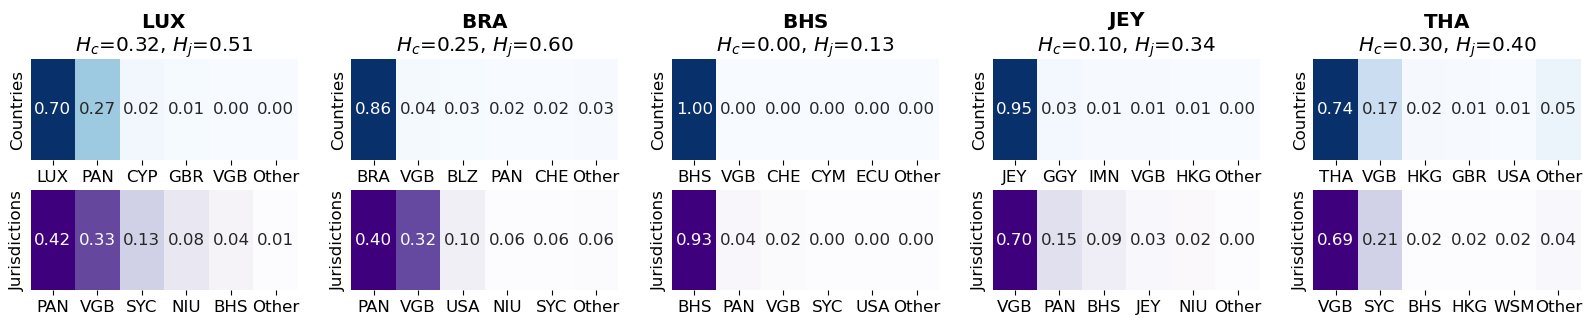
\includegraphics[width=0.8\textwidth]{Geography_Country_Heatmaps_Top11_15.png}
    \label{fig:geography_country_heatmaps_top11_15}
\end{figure}

\begin{figure}[htbp]
    \centering
    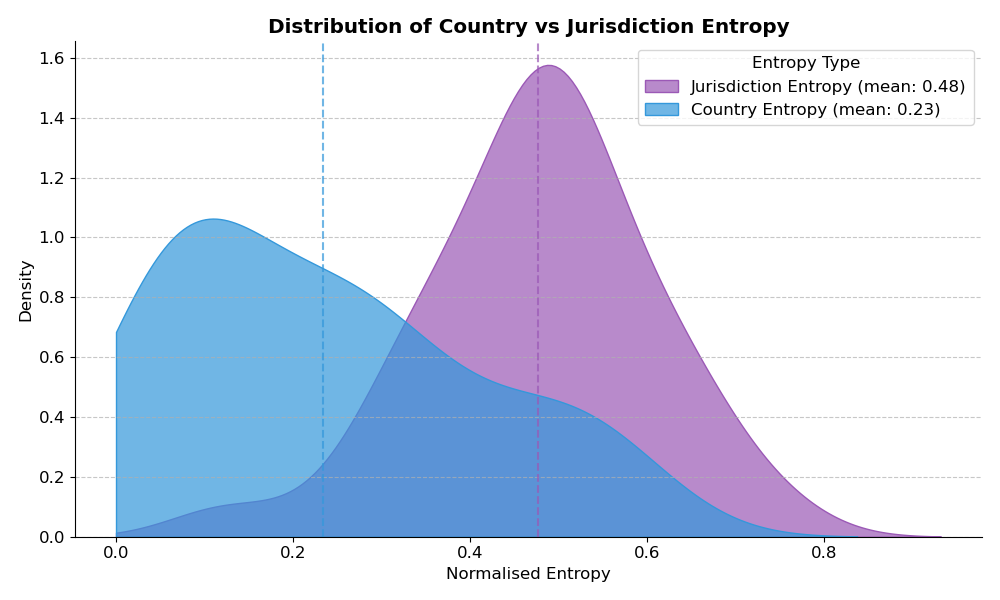
\includegraphics[width=0.8\textwidth]{Geography_Country_Level_Entropy_Distribution.png}
    \caption{Distribution of Entropy for Client Countries vs. Incorporation Jurisdictions at the Country Level of Intermediaries}
    \label{fig:geography_country_level_entropy_distribution}
\end{figure}

An illustrative example is Cyprus (Figure \ref{fig:geography_country_heatmaps_cyprus}), which is well-documented for its strong links to Russia. While Russia is generally underrepresented in the broader dataset, entities incorporated by Cypriot intermediaries show a significant Russian presence, with 12\% of such entities linked to Russia. This highlights a high lift for the Cyprus-Russia connection. Such specific high-lift pairs could be targets for further investigation, though that falls outside the scope of this thesis.

\begin{figure}[htbp]
    \centering
    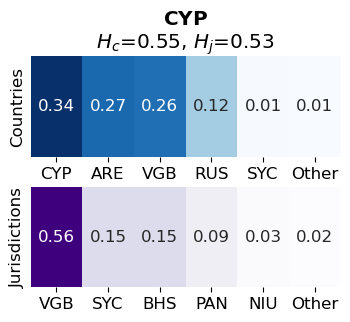
\includegraphics[width=0.8\textwidth]{Geography_Country_Heatmaps_Cyprus.png}
    \caption{Client and Incorporation Jurisdiction Heatmap for Cyprus-based Intermediaries}
    \label{fig:geography_country_heatmaps_cyprus}
\end{figure}

\subsubsection{Network of Countries Served by Intermediaries}
While intermediaries at the country level show specialisation, particularly in their client bases, this section examines the specific clusters of countries served by individual intermediaries. At the intermediary level, clientele also tends to be highly concentrated in one or two countries, as shown in Figure \ref{fig:geography_distribution_countries_by_intermediary}. Interestingly, even as intermediaries grow larger (i.e., serve more clients), there is a very low correlation between the number of clients served and the number of distinct countries their clients originate from.

\begin{figure}[htbp]
    \centering
    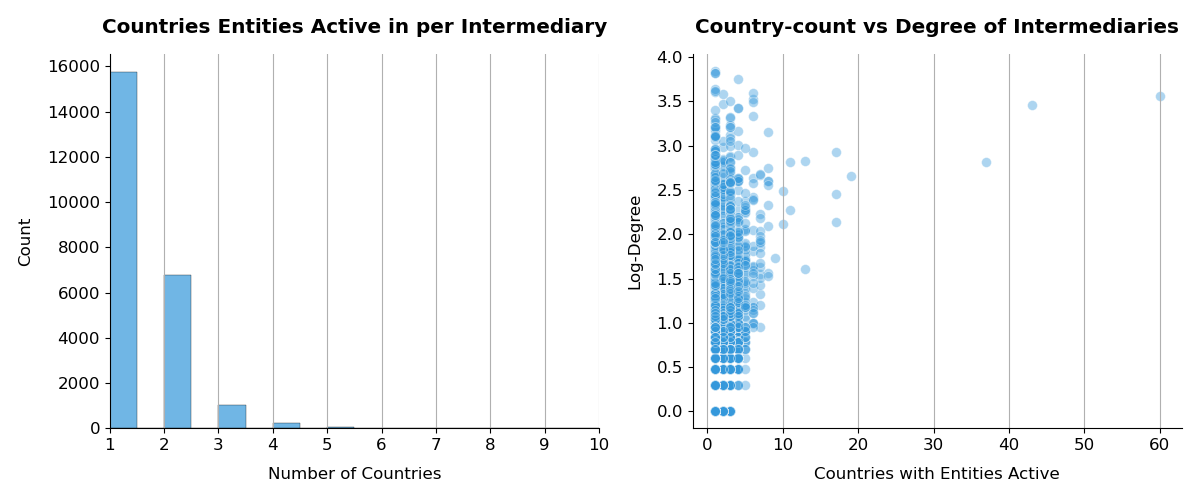
\includegraphics[width=0.8\textwidth]{Geography_Distribution_of_Countries_by_Intermediary.png}
    \caption{Distribution of the Number of Countries Served per Intermediary}
    \label{fig:geography_distribution_countries_by_intermediary}
\end{figure}

To explore these relationships further, a network of countries was constructed. In this network, two countries (nodes) are connected if an intermediary serves clients (entities) in both. The resulting full country network consists of 121 nodes and 2716 edges. Key summary statistics for this network are presented in Table \ref{tab:country_network_summary}.

\begin{table}[htbp]
\centering
\caption{Summary Statistics for the Full Country Co-Service Network}
\label{tab:country_network_summary}

\begin{tabular}{lc}
\toprule
Metric                        & Value    \\
\midrule
Number of Nodes               & 121      \\
Number of Edges               & 2716     \\
Network Density               & 0.3741   \\
Average Degree                & 44.89    \\
Average Clustering Coefficient & 0.7728   \\
\bottomrule
\end{tabular}
\end{table}

Visualising such dense graphs is challenging. Therefore, to identify the most important connections, the network was filtered using association analysis, as shown in Figure \ref{fig:geography_cross_country_network}. Edges are displayed only if they meet a support threshold (representing at least 0.008 of all intermediaries' country-pair connections) and a lift score of 1.5 or higher. This ensures that the visualized connections are not only frequent but also represent associations stronger than expected by chance. The resulting filtered network, or "backbone," thus highlights the most robust and significant co-service relationships. (The filtered graph presented features 14 clearly identifiable nodes: USA, BMU, CHN, HKG, CYM, VGB, SGP, TWN, MYS, COK, IDN, PAN, SYC, BHS, with WSM likely being the 15th implicitly).

The nodes in the network visualization are coloured in two ways: first, by communities identified using the Louvain method; and second, by regime type (VDem data). This was to explore whether regime type influences intermediary operations, though it appears less significant than other factors.

\begin{figure}[htbp]
    \centering
    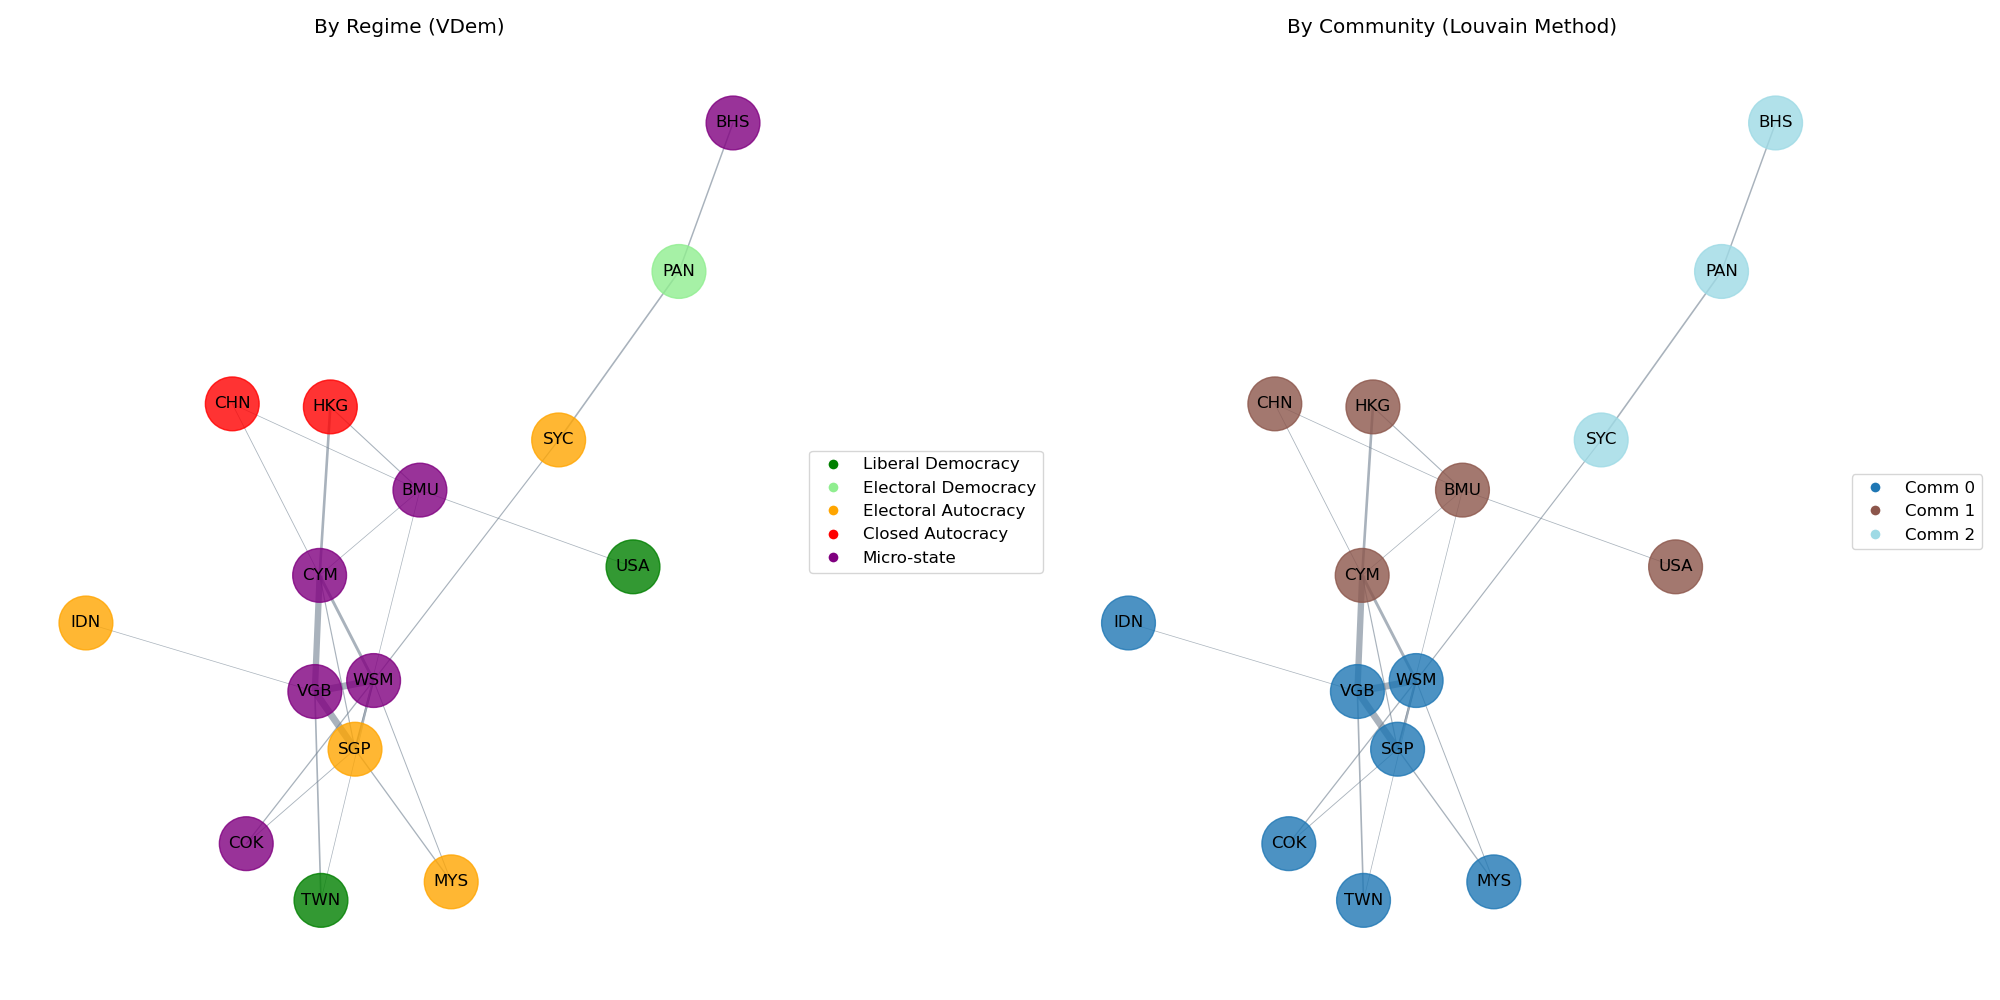
\includegraphics[width=0.9\textwidth]{Geography_Cross_Country_Network.png}
    \caption{Filtered Network of Co-Served Countries, Coloured by Louvain Community and Regime Type. Edges shown have support $\ge 0.008$ and lift $\ge 1.5$.}
    \label{fig:geography_cross_country_network}
\end{figure}

\paragraph{Interpretation of the Filtered Country Network Structure}
The filtered network (Figure \ref{fig:geography_cross_country_network}) reveals a sparse yet highly structured set of relationships. A central core of interconnected nodes is evident, particularly involving VGB (British Virgin Islands), CYM (Cayman Islands), SGP (Singapore), and their links to HKG (Hong Kong) and BMU (Bermuda).

When coloured by regime type, no clear large-scale clustering emerges. The central cluster itself includes Micro-states (VGB, CYM, BMU), Closed Autocracies (HKG), and Electoral Autocracies (SGP). Liberal Democracies like USA and TWN (Taiwan) are present but connect to nodes of different regime types. This visual evidence supports the notion that regime type is not a primary driver of these strong co-service relationships.

The Louvain community detection method reveals data-driven groupings:
\begin{itemize}
    \item \textbf{Community 0 (Dark Blue):} The largest, featuring VGB, SGP, CYM, TWN, MYS, IDN, COK (and likely WSM). This highlights strong ties between several offshore financial centers, key Asian economies, and Taiwan.
    \item \textbf{Community 1 (Brown):} Comprises USA, BMU, CHN, HKG, linking major economies with Bermuda.
    \item \textbf{Community 2 (Light Blue):} A smaller community of PAN, SYC, BHS.
\end{itemize}
Most nodes in this backbone are connected within 2-3 steps.

\paragraph{Centrality in the Country Network}
Centrality metrics for the full 121-node network (see Appendix Tables \ref{tab:appendix_country_betweenness} and \ref{tab:appendix_country_eigenvector}) identify key players.
\textbf{VGB (British Virgin Islands)} is dominant with the highest betweenness and eigenvector centrality. The \textbf{USA} ranks second in both, linked to BMU in the filtered graph's Community 1. \textbf{HKG \& CHN} also feature prominently in Community 1. Numerous \textbf{Micro-states} (BMU, BHS, CYM) show high centrality. \textbf{SGP (Singapore)} is another key, highly central node. High centrality in the full network generally translates to a significant structural role in this filtered backbone.

\paragraph{Significant Country Associations}
Lift scores from association analysis (Appendix Table \ref{tab:appendix_significant_country_associations}) reveal strong pairings (visualized in Figure \ref{fig:geography_cross_country_network} for lift $\ge 1.5$).
Key findings include:
\begin{itemize}
    \item Strong \textbf{Micro-state synergies} (e.g., VGB-CYM lift 1.91; CYM-BMU lift 13.47).
    \item A critical \textbf{USA-BMU-China/HKG nexus} (Comm 1): CHN-BMU (lift 15.28) and USA-BMU (lift 4.92) suggest Bermuda as a major intermediary hub for these powers.
    \item Robust \textbf{Asian connections} (e.g., SGP-MYS lift 5.27) and Singapore's links to Micro-states.
    \item A distinct \textbf{PAN-SYC-BHS nexus} (Comm 2).
    \item Crucially, high lift values are common \textbf{across different regime types}, reinforcing that factors beyond regime similarity (e.g., specialized services, legal systems) drive these strong ties.
\end{itemize}

\subsubsection{Network of Jurisdictions Used by Intermediaries}
Shifting focus to incorporation locations, this section analyzes the network of jurisdictions intermediaries use. The full jurisdiction network has 41 nodes and 347 edges (Summary statistics in Table \ref{tab:jurisdiction_network_summary}). Figure \ref{fig:geography_distribution_jurisdictions_by_intermediary} shows the distribution of jurisdictions used per intermediary.

\begin{table}[htbp]
\centering
\caption{Summary Statistics for the Full Jurisdiction Co-Usage Network}
\label{tab:jurisdiction_network_summary}
\begin{tabular}{lc}
\toprule
Metric                        & Value    \\
\midrule
Number of Nodes               & 41       \\
Number of Edges               & 347      \\
Network Density               & 0.4232   \\
Average Degree                & 16.93    \\
Average Clustering Coefficient & 0.8155   \\
\bottomrule
\end{tabular}
\end{table}

\begin{figure}[htbp]
    \centering
    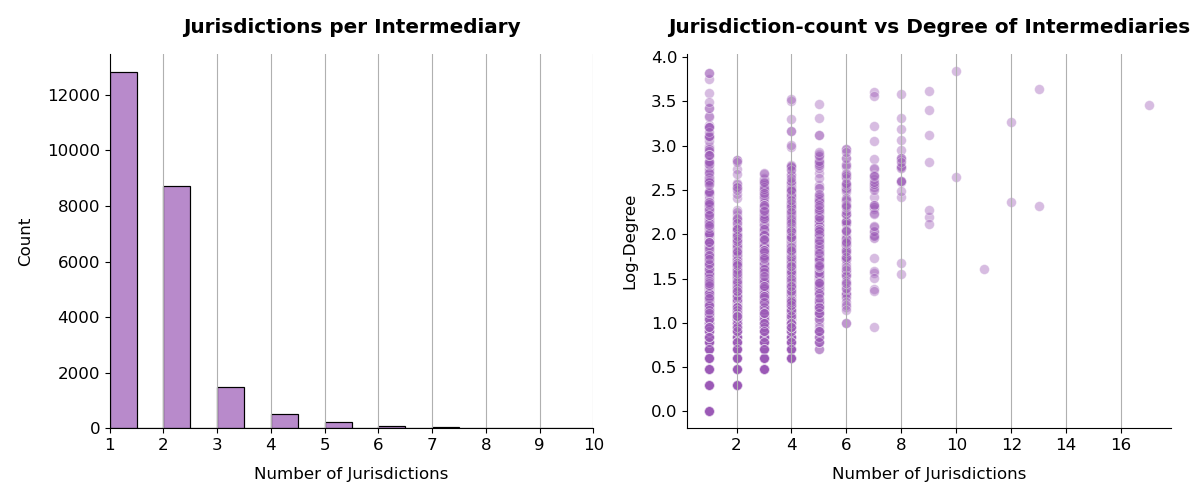
\includegraphics[width=0.8\textwidth]{Geography_Distribution_of_Jurisdictions_by_Intermediary.png}
    \caption{Distribution of the Number of Jurisdictions Used per Intermediary}
    \label{fig:geography_distribution_jurisdictions_by_intermediary}
\end{figure}

Figure \ref{fig:geography_cross_jurisdiction_network} presents a filtered "backbone" of co-usage patterns. Nodes are coloured by legal technology (Laffitte dataset) and Louvain communities. (The image shows 16 identifiable nodes: CRI, SGP, CYP, GBR, BLZ, AGO, HKG, CYM, COK, MYS, BHS, SYC, PAN, NIU, WSM, USA).

\begin{figure}[htbp]
    \centering
    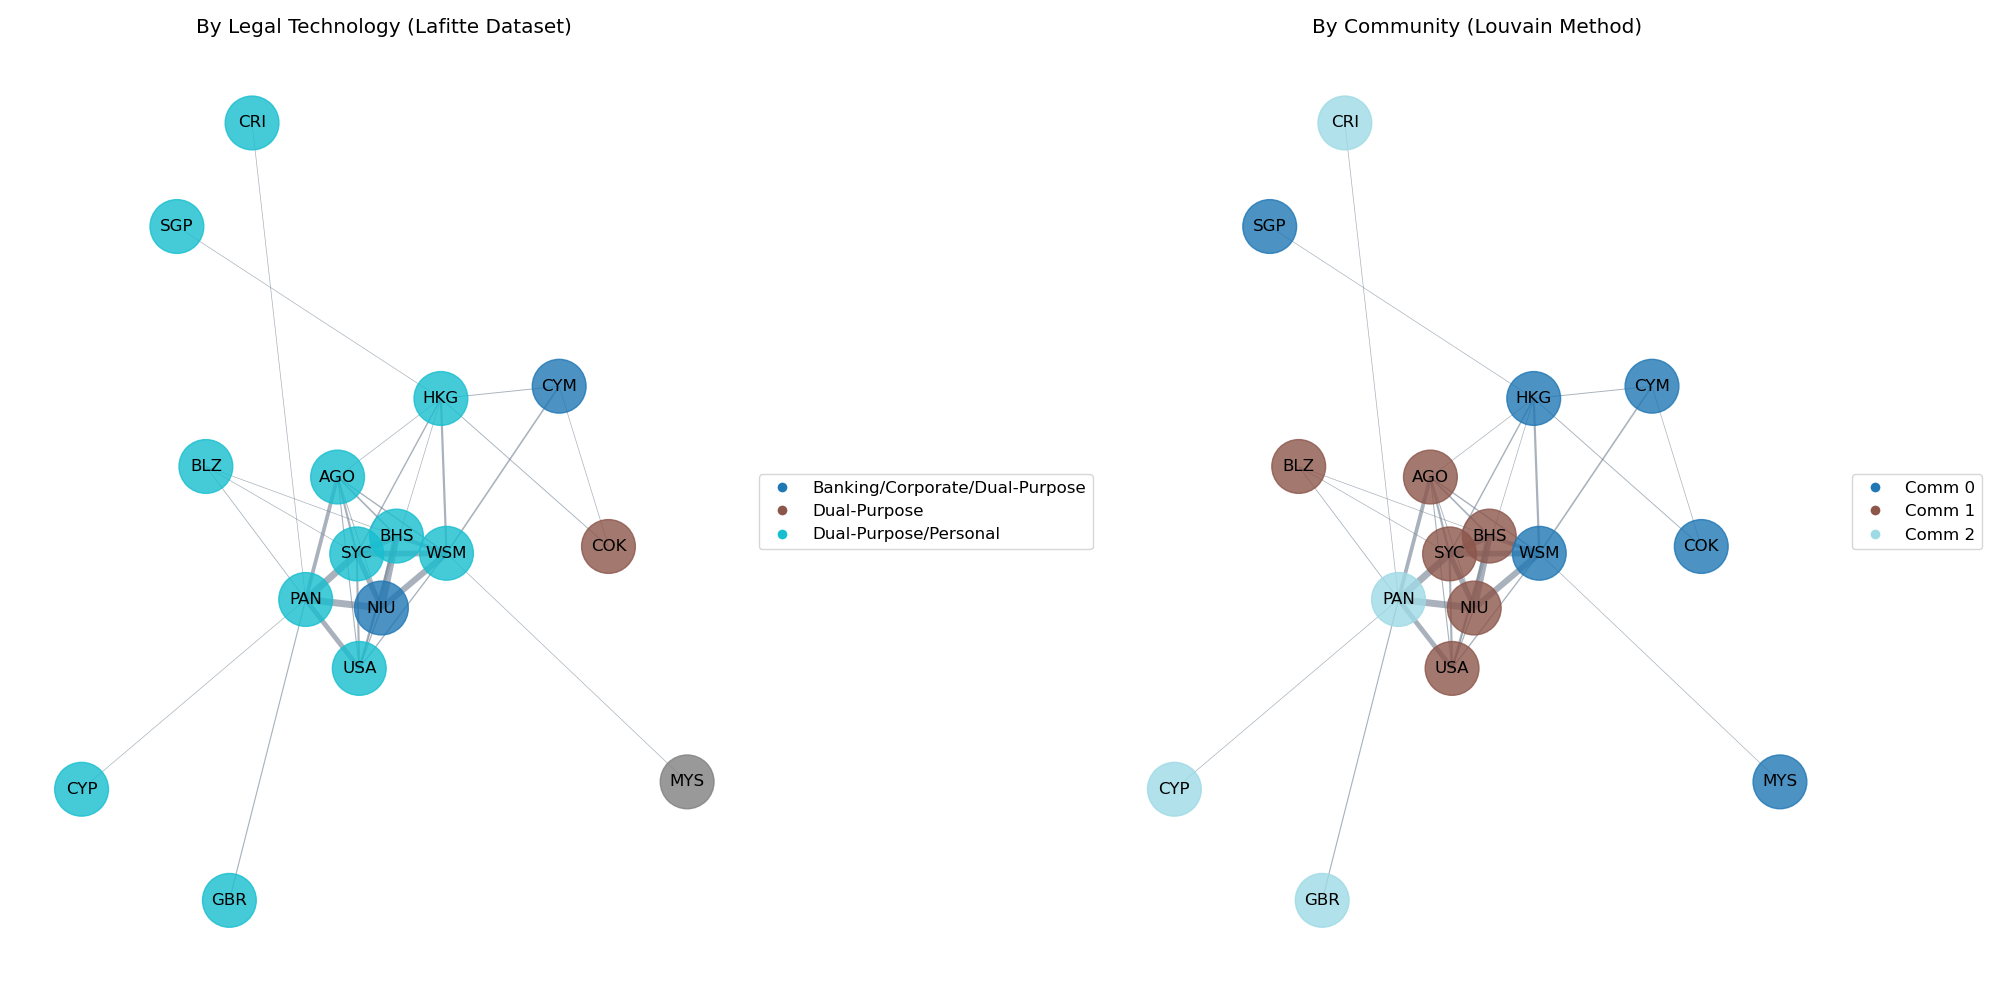
\includegraphics[width=0.9\textwidth]{Geography_Cross_Jurisdiction_Network.png}
    \caption{Filtered Network of Co-Used Jurisdictions, Coloured by Legal Technology and Louvain Community}
    \label{fig:geography_cross_jurisdiction_network}
\end{figure}

\paragraph{Interpretation of the Filtered Jurisdiction Network Structure}
The filtered jurisdiction network shows a central, densely connected core (BHS, SYC, AGO, WSM, NIU, PAN, USA, HKG).
Coloured by legal technology, the central cluster is dominated by jurisdictions offering \textbf{"Dual-Purpose"} legal technologies. This strongly supports the observation that central jurisdictions in this network tend to offer flexible, dual-purpose structures.

Louvain community detection identifies:
\begin{itemize}
    \item \textbf{Community 1 (Brown):} Largest and most central (USA, PAN, NIU, BHS, SYC, AGO, WSM), largely "Dual-Purpose" jurisdictions.
    \item \textbf{Community 0 (Dark Blue):} HKG, CYM, COK, combining "Banking/Corporate/Dual-Purpose" with "Dual-Purpose/Personal".
    \item \textbf{Community 2 (Light Blue):} More peripheral (SGP, CRI, CYP, GBR, BLZ, MYS).
\end{itemize}

\paragraph{Centrality in the Jurisdiction Network}
Centrality metrics for the full 41-jurisdiction network (Appendix Tables \ref{tab:appendix_jurisdiction_betweenness} and \ref{tab:appendix_jurisdiction_eigenvector}) are revealing.
\textbf{VGB (British Virgin Islands)} ranks \#1 in both betweenness and eigenvector centrality but is strikingly absent from the filtered graph. This implies its connections, while numerous, might not individually meet the high support/lift thresholds for this specific backbone view, or the visualization was capped.
\textbf{BHS (Bahamas)} and \textbf{PAN (Panama)} are 2nd and 3rd in centrality and visibly central in the filtered graph. \textbf{HKG} and \textbf{CYM} are also highly central and core to Comm 0. Most other top-ranked jurisdictions align with the backbone, with VGB being the main exception.

\paragraph{Significant Jurisdiction Associations}
Association analysis (Appendix Table \ref{tab:appendix_significant_jurisdiction_associations}) highlights strong co-usage:
\begin{itemize}
    \item The dominant \textbf{Community 1 ("Dual-Purpose" hubs)} shows very high mutual lift (e.g., BHS-NIU lift 4.64; NIU-WSM lift 5.33), with NIU as a critical connector.
    \item \textbf{Community 0 (financial centers)}: HKG-CYM (lift 5.82).
    \item Exceptional \textbf{cross-community lift}: AGO-BLZ (lift 20.41), suggesting specific niche relationships.
    \item High-lift associations often pair jurisdictions with \textbf{similar legal technology profiles}, but also occur between those with different profiles (e.g., WSM-CYM), indicating synergies drive co-usage.
    \item Peripheral jurisdictions (Comm 2) can have \textbf{extremely high lift values} in specific pairings (e.g., GBR-CRI lift 57.3; JEY-GGY lift 197!), pointing to highly specialized niches.
\end{itemize}

\subsection{Functional Specialisation of Intermediaries}
This section shifts from geography to the functional roles of intermediaries, exploring if a typology (e.g., EU, 2017; personalised advice vs. aid in incorporation) emerges. This analysis uses a classified random sample, as top-degree intermediaries aren't representative of the whole population (Figure \ref{fig:specialisation_classification_distribution}). The filtering of this sample is detailed in the Appendix (Figure \ref{fig:appendix_filtering_enrichment}).

\begin{figure}[htbp]
    \centering
    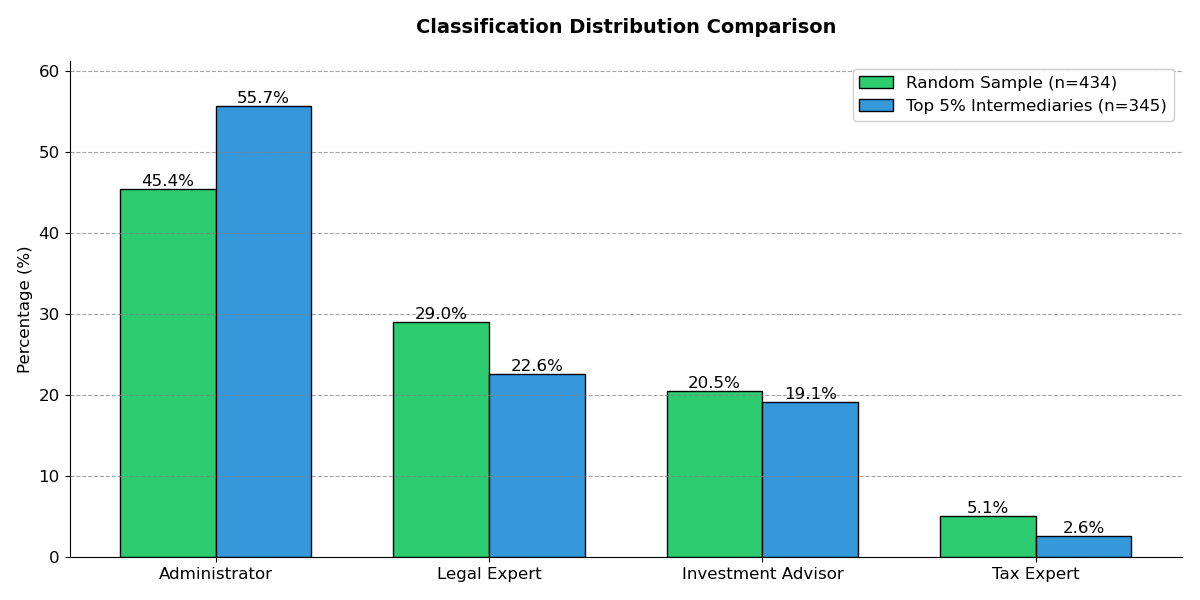
\includegraphics[width=0.8\textwidth]{Specialisation_Classification_Distribution_Comparison.png}
    \caption{Distribution of Intermediary Classifications}
    \label{fig:specialisation_classification_distribution}
\end{figure}

\begin{figure}[htbp]
    \centering
    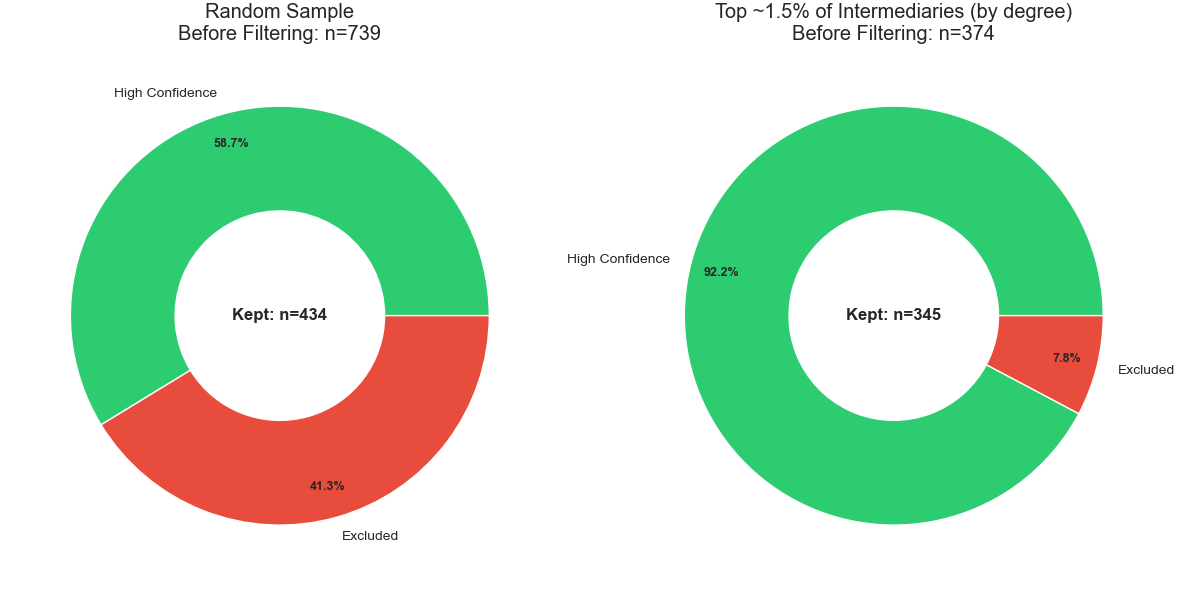
\includegraphics[width=0.8\textwidth]{Appendix_Filtering_of_Enrichment.png}
    \caption{Filtering Process of the Enriched Random Sample for Functional Classification}
    \label{fig:appendix_filtering_enrichment}
\end{figure}

\subsubsection{Different Levels of Connectivity: Personalised Advice vs. Aid in Incorporation}
A key differentiator is the number of entities incorporated. Administrators and legal experts appear more in top-degree intermediaries than tax experts/investment advisors. Figure \ref{fig:specialisation_cdf_degrees} shows the CDF of degrees by classification.

\begin{figure}[htbp]
    \centering
    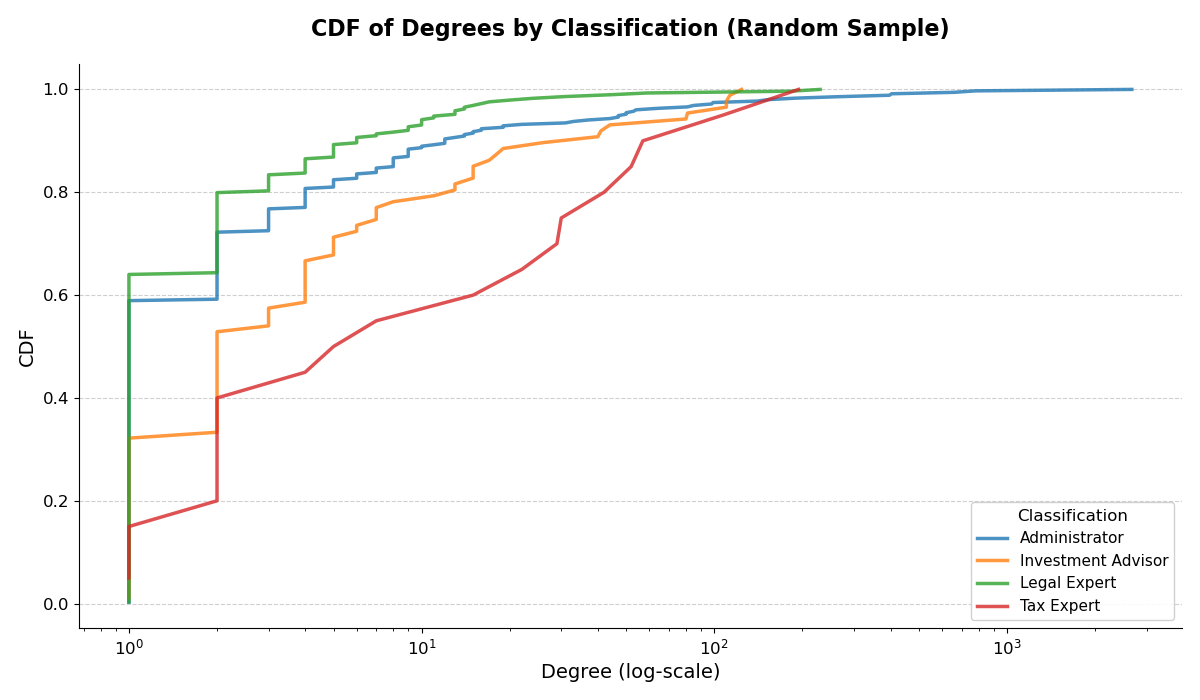
\includegraphics[width=0.8\textwidth]{Specialisation_CDF_of_Degrees_by_Classification_Random_Sample.png}
    \caption{CDF of Degrees by Intermediary Classification (Random Sample)}
    \label{fig:specialisation_cdf_degrees}
\end{figure}

Two-sample KS-tests (Bonferroni corrected for 6 pairs) found significant differences in degree distributions for 4 pairs. 'Tax Experts' and 'Investment Advisors' were not significantly different, nor were 'Legal Experts' and 'Administrators'. However, cross-group comparisons (e.g., 'Tax Experts' vs. 'Legal Experts') were all significant. This makes sense as the non-significant pairs are functionally more similar.

\subsubsection{Different Activities: Instruments and Service Offerings}
Intermediary activities are compared using five metrics:
\begin{enumerate}
    \item Entropy of incorporation jurisdictions.
    \item Entropy of client countries.
    \item Entropy of regimes of countries they incorporate in.
    \item Entropy of legal technologies in jurisdictions they incorporate in.
    \item Use of bearer instruments (binary).
\end{enumerate}
Figure \ref{fig:specialisation_average_entropy_bearer} shows average values by classification.

\begin{figure}[htbp]
    \centering
    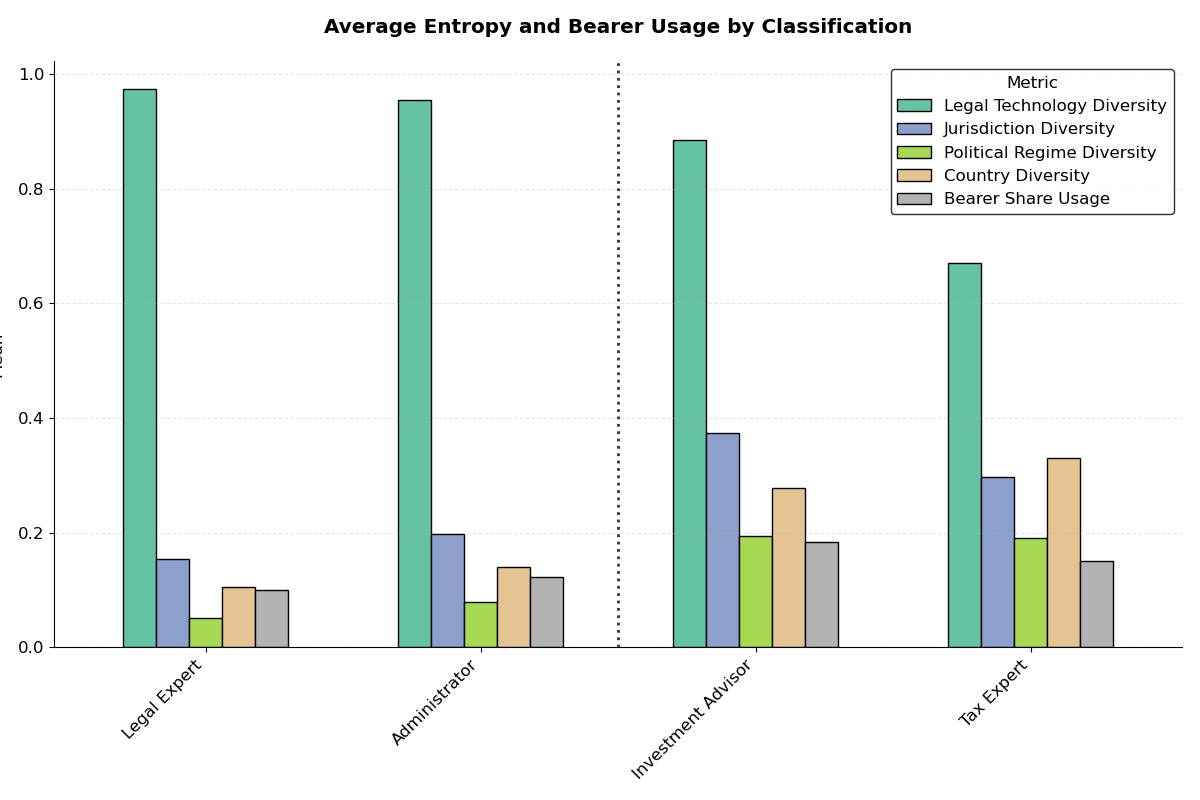
\includegraphics[width=0.8\textwidth]{Specialisation_Average_Entropy_and_Bearer_Usage_by_Classification.png}
    \caption{Average Entropy Measures and Bearer Instrument Usage by Intermediary Classification}
    \label{fig:specialisation_average_entropy_bearer}
\end{figure}

